\documentclass{article}
\usepackage[utf8x]{inputenc}
\usepackage{ucs}
\usepackage{amsmath} 
\usepackage{mathtext}
\usepackage{amsfonts}
\usepackage{upgreek}
\usepackage[english,russian]{babel}
\usepackage{graphicx}
\usepackage{float}
\usepackage{textcomp}
\usepackage{hyperref}
\usepackage{geometry}
  \geometry{left=2cm}
  \geometry{right=1.5cm}
  \geometry{top=1cm}
  \geometry{bottom=2cm}
\usepackage{tikz}
\usepackage{ccaption}
\usepackage{multicol}

\usepackage{listings}
%\setlength{\columnsep}{1.5cm}
%\setlength{\columnseprule}{0.2pt}


\begin{document}
\pagenumbering{gobble}

\lstset{
  language=C,                % choose the language of the code
  basicstyle=\linespread{1.1}\ttfamily,
  columns=fixed,
  fontadjust=true,
  basewidth=0.5em,
  keywordstyle=\color{blue}\bfseries,
  commentstyle=\color{gray},
  stringstyle=\ttfamily\color{orange!50!black},
  showstringspaces=false,
  %numbers=false,                   % where to put the line-numbers
  numbersep=5pt,
  numberstyle=\tiny\color{black},
  numberfirstline=true,
  stepnumber=1,                   % the step between two line-numbers.        
  numbersep=10pt,                  % how far the line-numbers are from the code
  backgroundcolor=\color{white},  % choose the background color. You must add \usepackage{color}
  showstringspaces=false,         % underline spaces within strings
  captionpos=b,                   % sets the caption-position to bottom
  breaklines=true,                % sets automatic line breaking
  breakatwhitespace=true,         % sets if automatic breaks should only happen at whitespace
  xleftmargin=.2in,
  extendedchars=\true,
  keepspaces = true,
}
\lstset{literate=%
   *{0}{{{\color{red!20!violet}0}}}1
    {1}{{{\color{red!20!violet}1}}}1
    {2}{{{\color{red!20!violet}2}}}1
    {3}{{{\color{red!20!violet}3}}}1
    {4}{{{\color{red!20!violet}4}}}1
    {5}{{{\color{red!20!violet}5}}}1
    {6}{{{\color{red!20!violet}6}}}1
    {7}{{{\color{red!20!violet}7}}}1
    {8}{{{\color{red!20!violet}8}}}1
    {9}{{{\color{red!20!violet}9}}}1
}

\section*{Повторение}
\begin{enumerate}



\item \textbf{Алгоритмы}
\begin{enumerate}
\item Заполните таблицу:
\begin{center}
  \begin{tabular}{ l || c }
    \hline
    Алгоритм & Сложность(в среднем) \\ \hline \hline
    Сортировка пузырьком & $O(n^2)$  \\ \hline
    Сортировка вставками &   \\ \hline
    Быстрая сортировка &   \\ \hline
    Цифровая сортировка & \\ \hline
    Простейший алгоритм перемножения матриц nxn & \\ \hline
    Добавление элемента в начало массива & \\ \hline
    Добавление элемента в начало связного списка & \\ \hline
  \end{tabular}
\end{center}

\item Предположим, что лучший алгоритм для задачи имеет сложность $O(N^2)$. К какому классу принадлежит данная задача (P или NP). То же самое для сложностей:
\begin{multicols}{3}
\begin{itemize}
\item $O(N^{10} + 5 N^{5})$.
\item $O(log(N))$.
\item $O(2^N)$
\end{itemize}
\end{multicols}

\item Машина Тьюринга: проведите вычисления для следующего примера:
\begin{figure}[H]
\centerline{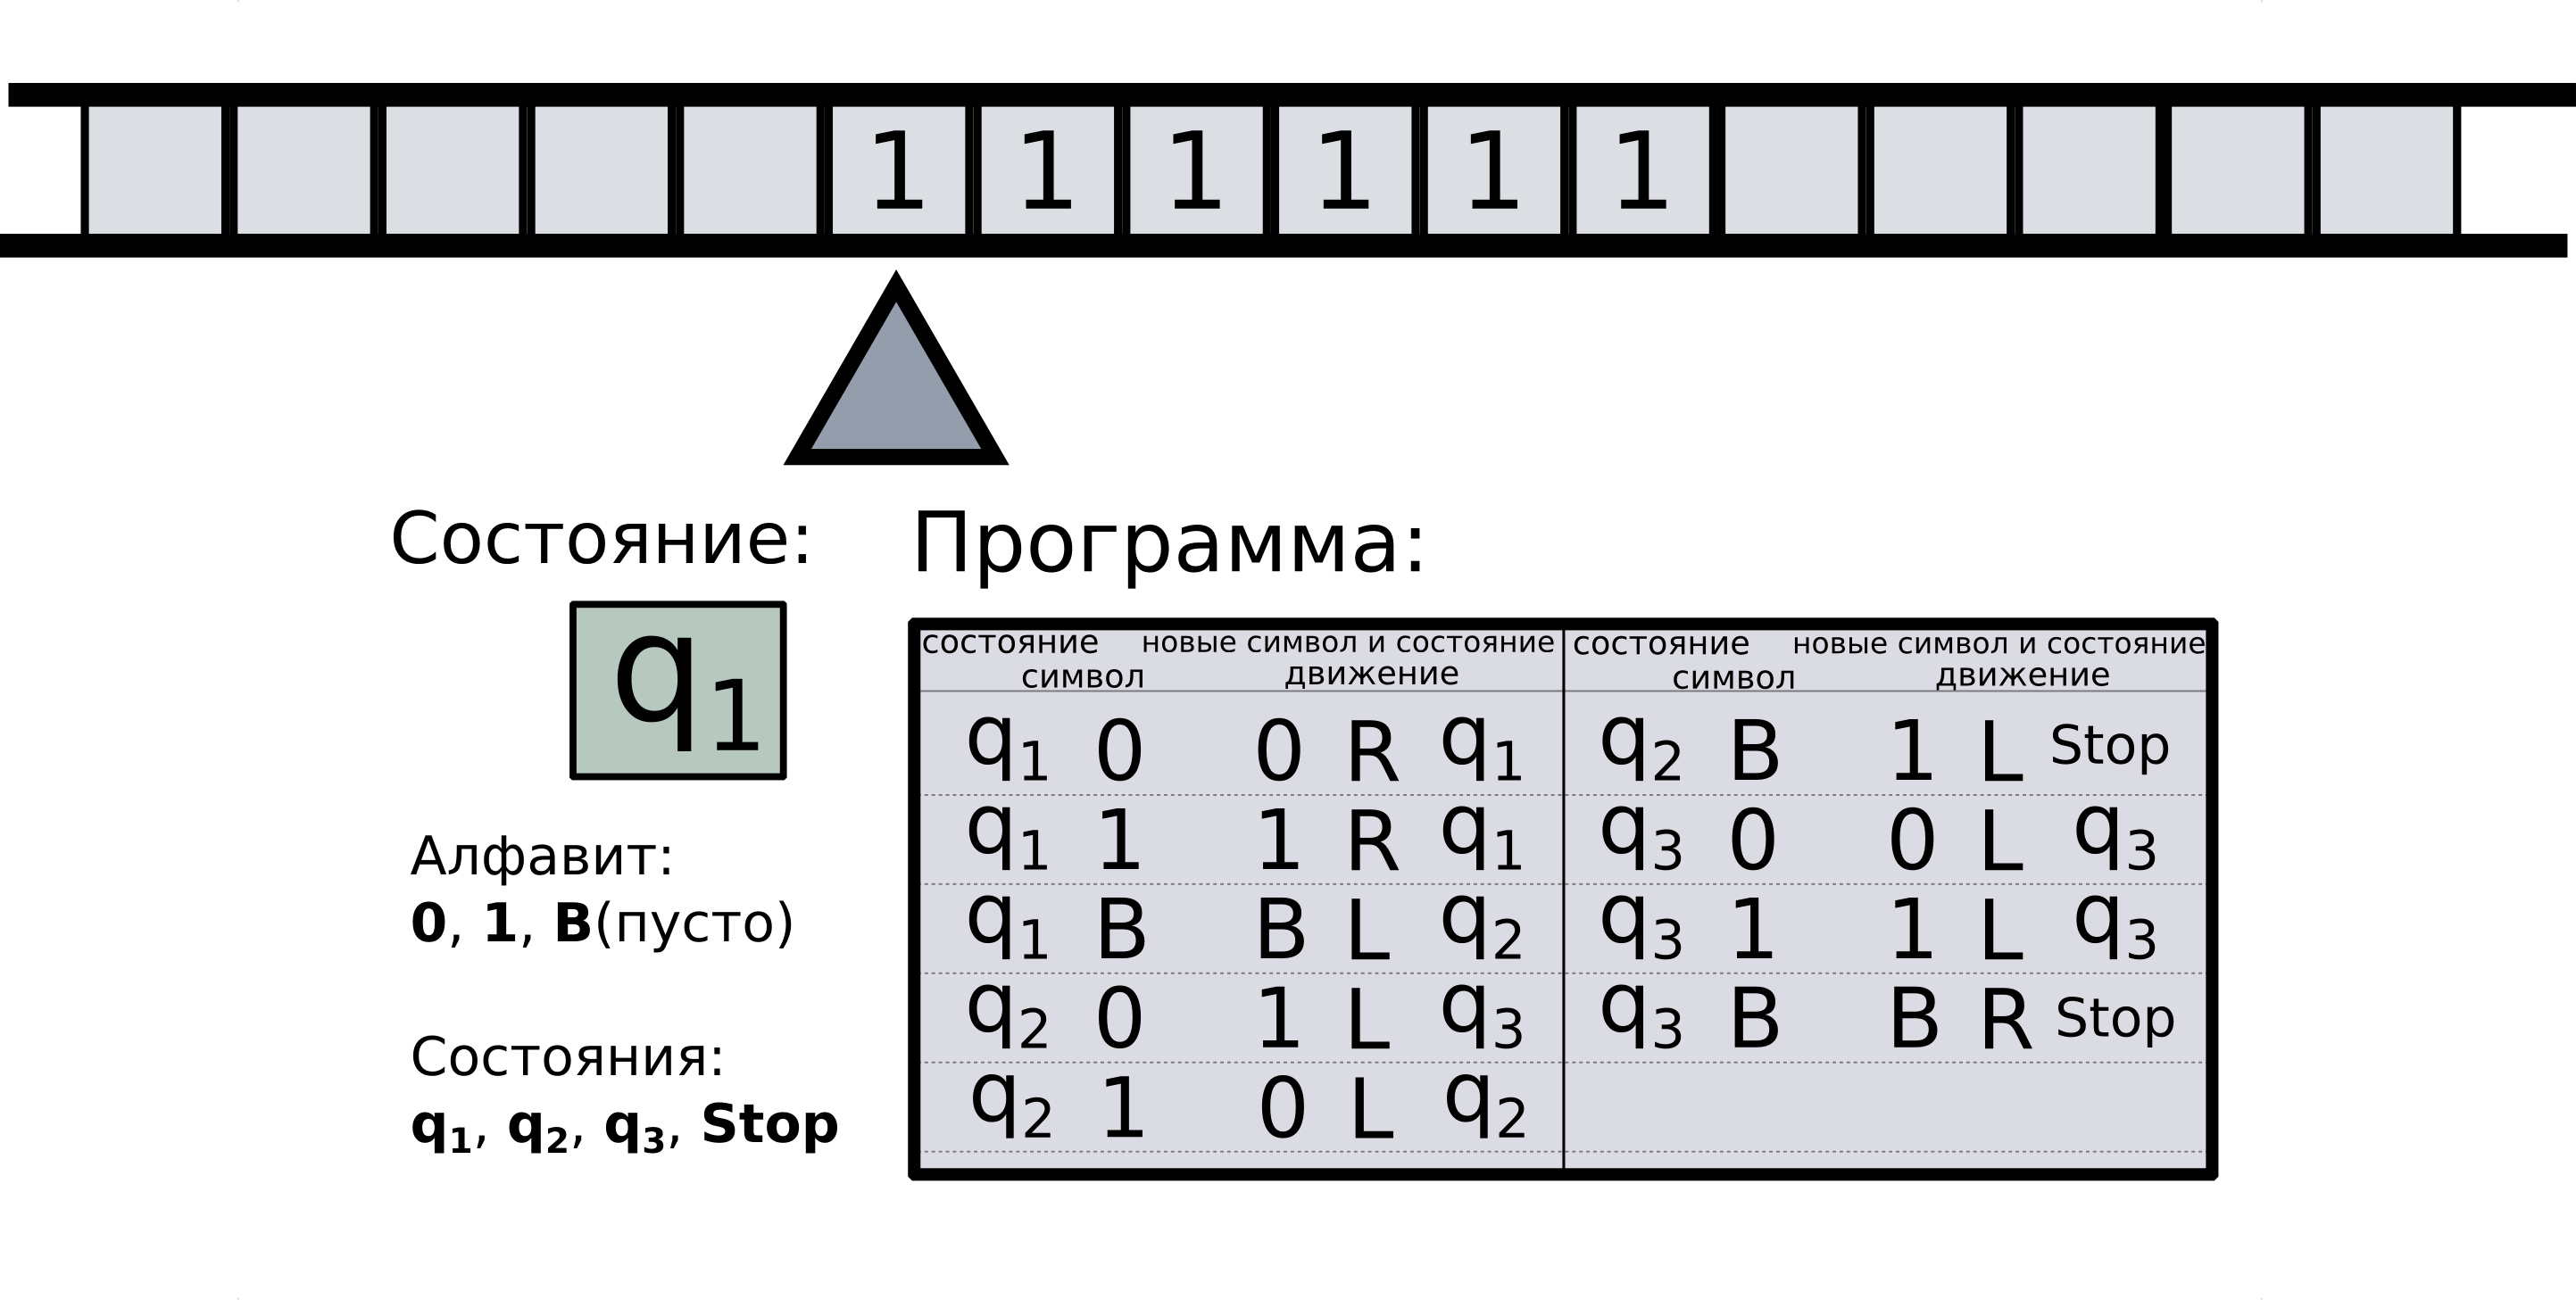
\includegraphics[width=0.7\linewidth]{tm.png}}
\end{figure}

\item Напишите программу для машины Тьюринга, которая умножает двоичное число на 2.


\item Класс NP это:
\begin{itemize}
\item Класс задач, которые нельзя решить за полиномиальное время на детерминированной машине Тьюринга.
\item Класс задач, которые можно решить за полиномиальное время  на недетерминированной машине Тьюринга.
\item Класс алгоритмов, которые нельзя выполнить за полиномиальное время на детерминированной машине Тьюринга.
\item Класс алгоритмов, которые можно выполнить за полиномиальное время на недетерминированной машине Тьюринга.
\end{itemize}
\end{enumerate}

\newpage

\item \textbf{Основы командной строки}
\begin{itemize}
\item \texttt{pwd} -- печать текущей директории
\item \texttt{ls <имя директории>} -- просмотр директории
\item \texttt{cd <имя директории>} -- переход в другую директорию
\item \texttt{mkdir <имя директории>} -- создать директорию
\item \texttt{subl <имя файла>} или \texttt{nano <имя файла>} -- открыть файл в соответствующем текстовом редакторе.
\item \texttt{.} -- текущая папка \quad \texttt{..} -- родительская папка \quad \texttt{/} -- корневая папка (аналог C:\ в windows) \quad тильда -- домашняя папка.
\item \texttt{top} -- диспетчер задач (выйти Ctrl-C).
\item \texttt{gcc <code.c>} -- компиляция кода из файла \texttt{code.c}
\item \texttt{./<имя программы>} -- запуск программы\\
\end{itemize}
\begin{enumerate}
\item Откройте терминал и перейдите в домашнюю папку (\texttt{/home-local/student}).
\item Создайте свою папку в этой директории и перейдите в неё.
\item Создайте простейшую программу и скомпилируйте её, используя gcc.
\end{enumerate}



\item \textbf{Основы C: переменные, массивы, функции, структуры, указатели}
\begin{enumerate}
\item Объявите переменную типа double и присвойте ей значение 2.718281828.
\item Объявите статический массив переменных типа int размера 6 элементов и инициализируйте его следующими значениями: 4, 8, 15, 16, 23, 42. (решение -- 1 строка)
\item Создайте динамический массив переменных типа int размера 6 элементов и инициализируйте его теми же значениями. (используйте malloc() и free() из \texttt{stdlib.h}).
\item Создайте функцию \texttt{float geometric\_mean(float a, float b)}, которая вычисляет геометрическое среднее. Не забудьте подключить математическую библиотеку: \texttt{math.h}, а также добавить опцию \texttt{-lm} при компиляции.
\item Опишите структуру \texttt{Complex}, описывающую комплексное число.
\item Напишите функцию \texttt{Complex complex\_add(Complex a, Complex b)}, которая складывает комплексные числа. Проверьте работу функции.
\item Напишите функцию \texttt{void complex\_sqr(Complex* pc)}, которая возводит комплексное число в квадрат. Проверьте работу функции на таком тесте: $(3 + 2i)^2 = 5 + 12i$.
\item Создайте новый файл \texttt{complex.h} и перенесите всё описание \texttt{Complex} в этот файл. Подключите этот файл к основному с помощью \texttt{\#include "complex.h"}.
\item Добавьте новые функции для работы со структурой \texttt{Complex} в файл \texttt{complex.h}.
\end{enumerate}

\end{enumerate}


\end{document}